
\setcounter{section}{0}
\textbf{Momen lực}

Momen lực $M$ đối với một trục quay là đại lượng đặc trưng cho tác dụng làm quay của lực $F$ và được đo bằng tích của lực với cánh tay đòn của nó. Công thức đặc trưng cho momen lực là 
\begin{equation*}
	M = F\cdot d, \label{eq1}
\end{equation*}
trong đó: 
\begin{itemize}
	\item $M$ là momen lực ($\textrm{Nm}$), 
	\item $F$ là lực đang xét ($\textrm{N}$),
	\item $d$ là cánh tay đòn của lực $F$ ($\textrm{m}$).
\end{itemize}

\textbf{Điều kiện cân bằng của một vật có trục quay cố định (Quy tắc momen lực)}

Muốn cho một vật có trục quay cố định ở trạng thái cân bằng thì tổng các moment lực có xung hướng làm vật quay theo chiều kim đồng hồ phải bằng tổng các momen lực có xu hướng làm vật quay ngược chiều kim đồng hồ.

\begin{center}
	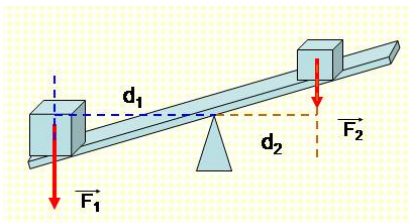
\includegraphics[scale=0.5]{../figs/VN10-PH-21-L-016-2-V2-01.png}
\end{center}

Nếu xét đến hai lực cùng tác dụng vào một vật có trục quay cố định thì vật ở trạng thái cân bằng khi

\begin{equation*}
	M_1 = M_2,
\end{equation*}
%
hay
%
\begin{equation*}
	F_1\cdot d_1 = F_2\cdot d_2. \label{eq2}
\end{equation*}
%
Nếu xét đến nhiều lực cùng tác dụng vào một vật có trục quay cố định thì vật ở trạng thái cân bằng khi
%
\begin{equation*}
	M_1+M_2+... = M'_1+M'_2+... 
\end{equation*}
%
\begin{equation*}
	F_1\cdot d_1+F_2\cdot d_2 + ... = F'_1\cdot d'_1 + F'_2\cdot d'_2+...
\end{equation*}
%
\luuy{Quy tắc momen lực còn được áp dụng cho cả trường hợp một vật không có trục quay cố định nếu như trong một tình huống cụ thể nào đó ở vật xuất hiện trục quay. }
\section{Trắc nghiệm}
\begin{enumerate}[label=\bfseries Câu \arabic*:]
	
	\item \mkstar{1}
	
	
	{Lực tác dụng vào vật làm cho vật quay quanh một trục có giá
		\begin{mcq}
			\item song song với trục quay.
			\item cắt trục quay.
			\item nằm trong mặt phẳng song song với trục quay.
			\item nằm trong mặt phẳng vuông góc với trục quay và không cắt trục quay.
		\end{mcq}
	}
	
	\hideall
	{	\textbf{Đáp án: D.}
		
		Lực tác dụng vào vật làm cho vật quay quanh một trục có giá nằm trong mặt phẳng vuông góc với trục quay và không cắt trục quay.
	}
		\item \mkstar{1}
	
	
	{Một ngẫu lực gồm có hai lực $\vec F_1$ và $\vec F_2$ có $F_1 = F_2 = F$ và có cánh tay đòn $d$. Momen ngẫu lực này là
		\begin{mcq}(2)
			\item $(F_1-F_2)d$.
			\item $2Fd$.
			\item $Fd$.
			\item Chưa xác định.
		\end{mcq}
	}
	
	\hideall
	{	\textbf{Đáp án: C.}
		
	}
		\item \mkstar{2}
	
	
	{Hai lực của ngẫu lực có độ lớn $F=\SI{20}{N}$, khoảng cách giữa hai giá của ngẫu lực là $d=\SI{30}{cm}$. Momen của ngẫu lực có độ lớn bằng
		\begin{mcq}(4)
			\item $\SI{0.6}{N.m}$.
			\item $\SI{600}{N.m}$.
			\item $\SI{6}{N.m}$.
			\item $\SI{60}{N.m}$.
		\end{mcq}
	}
	
	\hideall
	{	\textbf{Đáp án: C.}
		
		Momen của ngẫu lực:
		$$M=Fd = \SI{6}{N.m}$$
	}

	\item \mkstar{3}
	
	
	{Một thanh nhẹ gắn vào sàn tại B như hình vẽ.
		\begin{center}
			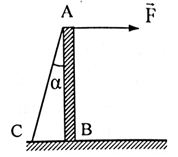
\includegraphics[scale=1]{../figs/VN10-2021-PH-TP021-6.png}
		\end{center}
		Tác dụng lên đầu A lực kéo $F=\SI{100}{N}$ theo phương ngang. Thanh được giữ cân bằng nhờ dây AC. Lực căng của dây có giá trị là bao nhiêu? Biết $\alpha = 30^\circ$.
		\begin{mcq}(4)
			\item $\SI{250}{N}$.
			\item $\SI{150}{N}$.
			\item $\SI{100}{N}$.
			\item $\SI{200}{N}$.
		\end{mcq}
	}
	
	\hideall
	{	\textbf{Đáp án: D.}	
		
		Chọn trục quay tại B. Áp dụng quy tắc momen lực:
		$$F \cdot \text{AB} = T \cdot \text{AB} \cdot \sin \alpha \Rightarrow T = \dfrac{F}{\sin \alpha} = \SI{200}{N}$$
	}
	
	
	
	\item \mkstar{4}
	
	
	{Bán cầu đồng chất khối lượng $\SI{100}{g}$. Trên mép bán cầu đặt một vật nhỏ khối lượng $\SI{7.5}{g}$. Hỏi mặt phẳng của bán cầu sẽ nghiêng góc $\alpha$ bao nhiêu khi nó cân bằng? Biết rằng trọng tâm bán cầu cách mặt phẳng của bán cầu một đoạn $3R/8$ (với $R$ là bán kính của bán cầu).
		\begin{center}
			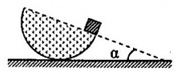
\includegraphics[scale=1]{../figs/VN10-2021-PH-TP021-7.png}
		\end{center}
		\begin{mcq}(4)
			\item $11,31^\circ$.
			\item $15^\circ$.
			\item $20^\circ$.
			\item $12^\circ$.
		\end{mcq}
	}
	
	\hideall
	{	\textbf{Đáp án: A.}
		
		\begin{center}
			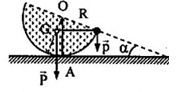
\includegraphics[scale=1]{../figs/VN10-2021-PH-TP021-8.png}
		\end{center}
		
		Các lực tác dụng lên bán cầu: trọng lực $\vec P$ của bán cầu, trọng lực $\vec p$ của vật nhỏ, phản lực $\vec Q$ tại điểm tiếp xúc A.
		
		Áp dụng quy tắc momen lực với trục quay qua O:
		$$P \cdot \text{OG} \cdot \sin \alpha = p \cdot R \cdot \cos \alpha \Rightarrow \tan \alpha = \dfrac{8m}{3M} \Rightarrow \alpha = 11,31^\circ$$
	}
	
	
\end{enumerate}



\hideall
{
	\begin{center}
		\textbf{BẢNG ĐÁP ÁN}
	\end{center}
	\begin{center}
		\begin{tabular}{|m{2.8em}|m{2.8em}|m{2.8em}|m{2.8em}|m{2.8em}|m{2.8em}|m{2.8em}|m{2.8em}|m{2.8em}|m{2.8em}|}
			\hline
			1.D  & 2.C  & 3.C & 4.D & 5.A  & & & & &  \\
			\hline
			
		\end{tabular}
	\end{center}
}
\section{Tự luận}
\begin{enumerate}[label=\bfseries Câu \arabic*:]
	\item \mkstar{1}
	
	{
		Momen lực đối với một trục quay là gì? Phát biểu điều kiện cân bằng của một vật có trục quay cố định (hay quy tắc momen lực).
	}
	
	\hideall{
		Momen lực đối với một trục quay là đại lượng đặc trưng cho tác dụng làm quay của lực và được đo bằng tích của lực với cánh tay đòn của nó.
		$$M=Fd,$$
		trong đó:
		\begin{itemize}
			\item $F$ là lực tác dụng $(\SI{}{N})$;
			\item $d$ là cánh tay đòn (là khoảng cách từ giá của lực đến trục quay) $\SI{}{m}$.
		\end{itemize}
		
		Muốn một vật có trục quay cố định nằm cân bằng thì tổng các momen lực có xu hướng làm cho vật quay theo chiều kim đồng hồ phải bằng tổng các momen lực có xu hướng làm cho vật quay ngược chiều kim đồng hồ.
	}
	
	\item \mkstar{2}
	
	
	{Hãy giải thích hoạt động của chiếc cân (hình vẽ).
		\begin{center}
			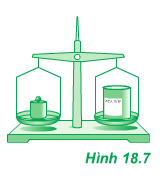
\includegraphics[scale=1]{../figs/VN10-2021-PH-TP021-5.png}
		\end{center}
	}
	
	\hideall
	{
		Khi cân nằm cân bằng (kim chỉ thẳng đứng), theo quy tắc momen lực, ta có:
		$$P_\text{vật} d_1 = P_\text{cân} d_2$$
		
		Vì $d_1=d_2$ nên khi đó $P_\text{vật} = P_\text{cân}$. Suy ra khối lượng vật cần đo bằng khối lượng của quả cân.
		
		Cân hoạt động theo quy tắc momen lực.
	}
	\item \mkstar{3}
	
	
	{Một người dùng búa để nhổ một chiếc đinh, khi người đó tác dụng một lực $\SI{50}{N}$ vào đầu búa thì đinh bắt chuyển động. Biết cánh tay đòn của lực tác dụng của người đó là $\SI{20}{cm}$ và cánh tay đòn của lực nhổ đinh khỏi gỗ là $\SI{2}{cm}$. Hãy tính lực cản của gỗ tác dụng vào đinh.
	}
	
	\hideall
	{Gọi 
		\begin{itemize}
			\item $M_1$ và $M_2$ là momen lực do tay người và lực cản của gỗ tác dụng lên búa ($\textrm{Nm}$),
			\item $F_1$ là lực do tay người tác dụng vào đầu búa ($\textrm{N}$),
			\item $F_2$ là lực nhổ đinh, hay là lực cản của gỗ cây đinh lại ($\textrm{N}$), 
			\item  $d_1=\SI{20}{cm}$ là cánh tay đòn từ tay người đến trục quay ($\textrm{m}$), 
			\item  $d_2=\SI{2}{cm}$ là cánh tay đòn từ đinh đến trục quay ($\textrm{m}$). 
		\end{itemize}
		
		Khi đinh bắt đầu chuyển động, câu búa đang ở trạng thái cân bằng, nên ta áp dụng quy tắc momen lực
		%
		\begin{equation*}
			M_1=M_2 \Rightarrow F_1\cdot d_1 = F_2\cdot d_2
		\end{equation*}
		% 
		Từ đó, ta tính được lực cản của gỗ tác dụng vào đinh 
		%
		\begin{equation*}
			F_2=F_2\cdot \dfrac{d_1}{d_2}
			=
			\SI{50}{N}\cdot \dfrac{\SI{20}{cm}}{\SI{2}{cm}}
			=
			\SI{500}{N}.
		\end{equation*}
		%
		Vậy lực cản do miếng gỗ tác dụng lên cây đinh lúc đó là $F_2=\SI{500}{N}$.
	}
	\item \mkstar{4}
	
	
	{Một thanh gỗ dài $\SI{1,8}{m}$ nặng $\SI{30}{kg}$, một đầu được gắn vào trần nhà nhờ một bản lề, đầu còn lại được buộc vào một sợi dây và gắn vào trần nhà sao cho phương của sợi dây thẳng đứng và giữ cho tấm gỗ nằm nghiêng hợp với trần nhà nằm ngang một góc $45^{\circ}$. Biết trọng tâm của thanh gỗ cách đầu gắn sợi dây $\SI{60}{cm}$. Tính lực căng của sợi dây, lấy $g=\SI[parse-numbers=false]{10}{m/s^2}$.
		\begin{center}
			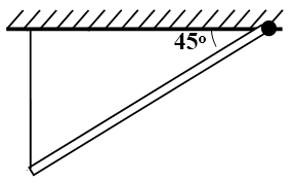
\includegraphics[scale=0.7]{../figs/VN10-2021-PH-TP021-1.png}
		\end{center} 
	}
	
	\hideall
	{Đầu tiên, ta quy định các đại lượng trong bài toán và xác định cánh tay đòn như sau: 
		\begin{itemize}
			\item $T$ là lực căng của sợi dây tác dụng lên điểm A trên tấm gỗ, 
			\item $P=m\cdot g= \SI{30}{kg} = \SI{300}{N}$ là trọng lực tác dụng lên tấm gỗ tại trọng tâm G, 
			\item $\alpha = 45^{\circ}$ là góc hợp bởi tấm gỗ và trần nhà, 
			\item $d$ là khoảng cách từ điểm G đến trục quay O,
			\item $d'$ là khoảng cách từ điểm treo của dây đến trục quay O,
			\item $l=\SI{1,8}{m}$ là chiều dài của thanh gỗ. 
		\end{itemize}
		%--------------------------------%
		\begin{center}
			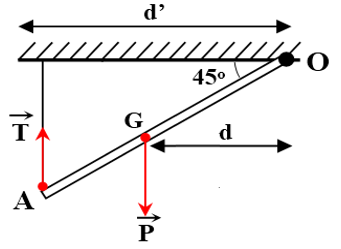
\includegraphics[scale=0.7]{../figs/VN10-2021-PH-TP021-2.png}
		\end{center}
		Tiếp theo, ta tính độ dài các cánh tay đòn bằng cách áp dụng công thức \eqref{ctd}. Cánh tay đòn của trọng lực là
		\begin{equation*}
			d=\textrm{OG}\cdot\cos 45^{\circ}=\dfrac{1}{2}\cdot \SI{1,8}{m}\cdot \cos 45^{\circ}.
		\end{equation*}
		%
		Cánh tay đòn tương ứng với lực căng dây là
		\begin{equation*}
			d' = \textrm{OA}\cdot \cos 45^{\circ} =\SI{1,8}{m}\cdot \cos 45^{\circ}.
		\end{equation*}
		%
		Áp dụng quy tắc momen lực, ta có
		\begin{align*}
			T\cdot d' &= P\cdot d\\
			\Rightarrow
			T&=\dfrac{P\cdot d}{ d'}
			=
			\dfrac{\SI{300}{N}\cdot \dfrac{1}{2}\cdot \SI{1,8}{m}\cdot \cos 45^{\circ}}{\SI{1,8}{m}\cdot \cos 45^{\circ}}
			=\SI{150}{N}
		\end{align*}
		Vậy lực căng dây là $T=\SI{150}{N}$. 
	}
		\item \mkstar{4}
	
	
	{Một vật rắn phẳng, mỏng, có dạng là một hình vuông ABCD, mỗi cạnh là $a=\SI{10}{cm}$. Người ta tác dụng một ngẫu lực nằm trong mặt phẳng của hình vuông. Biết các lực vuông góc với đường chéo AD có độ lớn $\SI{10}{N}$ và đặt vào hai đỉnh của A và D. Tính momen của ngẫu lực.
	}
	
	\hideall
	{Ta có đường chéo của hình vuông:
		$$d=\sqrt{a^2 + a^2} = \SI{14.14}{cm} = \SI{0.14}{m}$$
		
		Momen ngẫu lực:
		$$M=Fd = \SI{1.41}{Nm}$$
	}
\end{enumerate}